% class definitions
\documentclass[a4paper,12pt]{scrartcl}

% Packages

\usepackage[utf8]{inputenc}
\usepackage[ngerman]{babel}
\usepackage[T1]{fontenc}
\usepackage{graphicx}
\usepackage{lmodern}
\usepackage{tabto}
\usepackage{listings}
\usepackage{quoting} %
\usepackage{lipsum}
\quotingsetup{font={itshape}, leftmargin=2em, rightmargin=0in, vskip=1ex}
\usepackage{framed} 
\usepackage{xcolor} 
\colorlet{shadecolor}{gray!25}

\usepackage[backend=biber, style=authoryear]{biblatex}


% Front page

\title{ Flubot:\\ Android-Malware verbreitet sich über Fake-Patches }
\subtitle{Cybersecurity}
\author{Moritz Rupp}
\date{Wintersemester 2021/22}


% Mathepakete
\usepackage{amsfonts}
\usepackage{amsmath}

%Document start 
\begin{document}
 


\maketitle
\newpage
\tableofcontents
\newpage


\section{Abstract}
Die tägliche Nutzung von Smartphones ist nunmehr seit über 10 Jahren in der breiten Geselschaft angekommen. Egal ob private oder geschäftliche  kurznachrichtendienste, Online Banking oder shopping. In allen Bereichen des sozialen und geschäftlichen Lebens finder das smartphone Anwendung. Auch neuere Erscheinungen wie der online handel mit crypto währungen findet breit über mobile endgeräte statt. \\
Derzeit sind laut der Musterquelle über 3 Milliarden mobile Geräte im Umlauf. Davon nutzt über die Hälfte das Betriebssystem Android.
Die große Anzahl an ähnlichen Geräten mit einer ähnlichen Software auf denen sensitive Daten laufen bietet eine Menge an Angriffsmöglichkeiten.
Phishing gilt seit jahren als eine der größten gefahren.
Meist durch imitation eines Anbieters oder Dienstes wird versucht Opfer eine externe Software zu installieren. Diese liest nun je nach Angriff belieb Daten aus.
Das ganze wird meist durch verschiedene Angriffsverktoren erreicht!
Unter anderem spielt Social engineering eine Rolle. 
Das ganze wird in einem Angrgiffsszenario kombiniert bzw. zusammengeführt!
Das Botnetz Flubot ist solch ein Phishing angriff und wird in dieser Arbeit untersucht.



\newpage
\section{Einführung}
Die Android-Malware 'Flubot' trat das erste mal Ende des Jahres 2020 auf. Anfangs \\hunderte, später tausende von Android Nutzern berichteten über eine Vielzahl von verdächtigen SMS Nachrichten. Zwar unterschieden sich die Mitteilungen in gewissen Details, jedoch war der Kernaufbau der Nachricht immer der gleiche. Ein kurzer Text, gefolgt von einem Link. In dem  Nachrichtentext wurde der Empfänger auf einen Dienst hingewießen der über den Link zu erreichen sei. Öffnete man diesen wurde man auf eine Webseite weitergeleitet. Hier sollte der jeweilige Dienst über ein Download nutzbar gemacht werden. Durch Installation dieses Downloads infizierte sich das Gerät mit Flubot. In folge dessen durchläuft die Malware das Adressbuch und verbreitet sich daraufhin namesgebend wie ein Flobefall über private Kontakte!\\
Anfangs stellte der Köder eine vermeintlich verpasste Voicemail da. Im weiteren Verlauf der Angriffe wurden zudem Packetlieferdienste imitiert die auf ein bald eintreffendes Packet aufmerksam machen sollten. 
Seit Mitte des Jahres 2021 wird nun versucht mit Sicherheitsupdates gegen Flubot selbst zu täuschen.\\
Für Branchenkenner war schnell klar das dass ganze eine groß Angelegte Phising Kampagne darstellte!\\ Aufgrund der Tatsache das Flubot nach wie vor im Umlauf ist lässt sich schwer einschätzen wie viele Geräte derzeit Infiziert sind. Im Deutschen Raum werden Schätzungen zwischen 1-3 Millionen Endgeräten laut. Auch finanziell ist die Schadenssumme derzeit nicht präzise zu bestimmen. Schätzen sprechen hier jedoch zwischen 4-8 Millarden Euro.\\
Durch diese Ausmaße führte Flubot zu einem neuen Bewustsein von Phising Angriffen.
Gegenstand dieser Arbeit ist es die Bedrohungslage von solch Angriffen zu verstehen und Lösungsansätze zu finden.\\
Dafür wird anfangs die Funktionsweiße genauer untersucht und erleutert.
Anschließend wird durch eine Technische Analyse die eigentliche Anwendung hinter Flubot aus Angreifersicht beleuchtet.\\
Darauf aufbauend werden nun verschiedene Lösungsansätze diskutiert und vorgeschlagen.
Abschließend werden die neu erlernten Kenntisse zusammengeführt und ein Ausblick in zukünftige Bedrohungslagen und Lösungen gewagt.
																					
\newpage
\section{Funktionsweiße}
\subsection{Infektion und Verbeitung}
Flubot lässt sich terminologisch als 'Banking Trojaner' einordnen. Das heißt Hauptintension der Schadware besteht darin als nützliches Programm getarnt in Geräte einzudringen und Banking Informationen abzugreifen. Die Infektion und Verbreitung von Trojaner werden häufig mithilfe von Botnetzen betrieben. Diese bestehen aus oftmals tausenden Geräten die automatisiert die Malware betreiben und sich zudem über das befallene Gerät weiter ausbreiten. 
Erste Handlung von solch Angriffen ist es also eine große Anzahl an potenziellen Opfern zu Kontaktieren.
Im Falle von Flubot wird davon ausgegangen das ein großteil der ersten  Mobilfunknummern durch einen Datenleak von Facebook stammen. Mitte  2020 war es Angreifern gelungen persönliche Profil-Daten mitsamt Handy Nummern von über 11 Millionen Britischen Facebook accounts abzugreifen. Des weiteren wurden höchstwahrscheinlich weitere Datenleaks der letzten Jahre genutzt!\\ 
Durch die Länder Vorwahl ist Flubot in der Lage aus einer Liste von Phishing Ködern zu wählen die zu Sprache und Region des Opfers passen.
Eine Phishing SMS setzte sich anfangs lediglich aus einer kurzen Nachricht und einem Link zusammen.
\begin{shaded}

 voice message received:
 hxxp://tantawy-group[.com/z.php?REDACTED
\end{shaded}
Nachdem jedoch viele dieser Nachrichten durch SMS-Filter seitens der Mobilfunkanbieter geblockt wurden, passte sich das Botnetz durch komplexere Meldungen an. Nun wurde ein prefix aus zufälligen Zahlen und Buchstaben vor der eigentlich Nachricht eingefügt. Auch im Nachrichtentext wurden teilweise einzelne Buchstaben geflipt.
Im Verlauf der Angriffe wechselten die Köder Nachrichten sehr häufig. So wurde vorallem im deutschsprachigen Raum  mit Packet Tracking Mitteilungen von DHL gearbeitet. In den USA meist mit Lieferdiensten wie Fedex und UPS. Zuletzt nun mit Sicherheitsupdates gegen Flubot selbst. Diese Nachrichten gaben vor eine Infektion des Gerätes erkannt zu haben die nur durch Installation externer Software entfernt werden könne.
\begin{shaded}
asdjljNew voice-message jecoived:
hxxp://fyqz[.vip/m.php?REDACTED\\
Ihr Packet kommt an, folgen sie es hier: https:proudhouseporpery:/64asdasd\\
DHL: Your parcel is arriving track here: asdadsajdladskjlkajda\\


\end{shaded}
In allen Fällen führt der Link auf eine Webseite. Auf dieser wird aufgefordert ein Android Package Kit herunterzuladen dass den jeweiligen Dienst nutzbar macht. Anhand einer kurzen Anleitung wird zudem gezeigt wie externe App Installationen zugelassen werden können. Nach Installation dieser APK ist das betroffene Gerät endgültig Infiziert und Teil des Botnetzes.\\


\newpage
\subsection{Post Infection}
Erste Handlung der Malware ist es nun eine Verbindung zu dem Command and Control Server aufzubauen. Dieser ist eine art Hauptzentrale der Malware Infrastrukur und steuert viele Abläufe der Angriffe. Auch gekapperte Daten werden hier in Datenbanken verschlüsselt gespeichert und weiterverabreitet. Ist die Verbindung hergestellt durchsucht Flubot das komplette Adressbuch des Infizierten Gerätes und sendet die Kontakte an den C\&C  Server. Dieser antwortet erneut mit einer Liste von Handy nummern die bereits durch andere Bots gesichert wurden. Über diese wird nun die Verbeitung der Malware fortgesetzt. Um eine Mustererkennung und Blockierung vorzubeugen verbreitet sich das Botnetz meist nur über neue Kontakte des C\&C Servers. 
\begin{center}
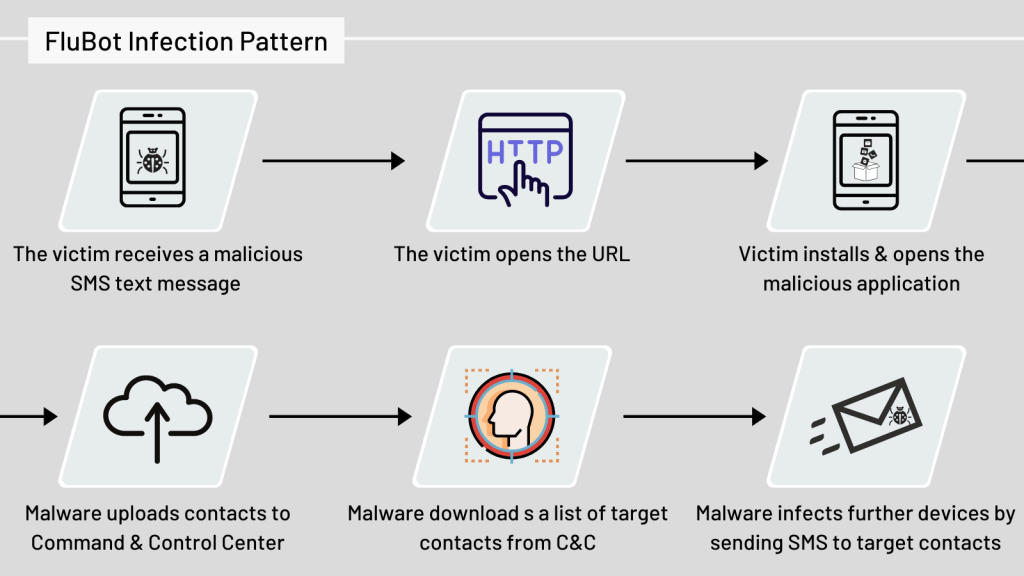
\includegraphics[scale=0.41]{command_control_server.png} 
\end{center}
Des weiteren schickt das Infizierte Gerät eine Liste der installierten Applicationen an den Command and Control Server. Dieser Antwortet wiederum mit einer Liste von Apps die komprementiert werden sollen. Größtenteils konzentriert sich Flubot auf Banking Apps, aus denen Login Informationen ausgelesen werden. Weitere Ziele sind Dienste für Kryptowährungen. Darunter auch sogenannte 'Multi-Asset-Broker. Also Dienstleister die den Handel mehrerer Vermögenswerte wie Aktien, ETFs oder auch Kryptowährungen anbieten. In allen Fällen werden die ausgewählten Anwendungen injeziert. Öffnet ein Opfer nun eine der betroffenen Apps liegt ein Phishing Overlay des Login Screens als Maske über der eigentlichen Anwendung.
Jegliche Eingaben werden nun an den C\&C Server weitergeleitet.
Weitere schädliche Aktionen beinhalten das deinstallieren von Apps, die unterbindung von benachrichtigungen und das Auslesen von Kreditkarten Informationen. Durch die Möglichkeit über den Command and control Server immer wieder auch neue Angriffe zu steuern bietet Flubot über den ursprünglichen Nutzen hinaus die Möglichkeit Profit aus dem infizierten Gerät zu generieren.



\newpage
\section{Technische Analyse}
\subsection{Netzwerkstrukur}
Hinter Flubot steckt eine großflächige Infrastrukur. Kern des ganzen bildet bekanntlich der Command and Control Server. Dieser liegt nicht fest auf einem Webspace sondern arbeitet als verteiltes System auf mehreren hundert Instanzen. Kompromitierte Webseiten wie Wordpress Blogs dienen hierbei als Hosts. In früheren Botnetzen lag der C\&C Server fest auf einer dedizierten Domäne. Dies war einfach zu bekämpfen, da nach Ermittlung der IP Adresse der Internet-Service Provider diese Blockieren konnte und somit die Verbreitung des Botnetzes stoppte. Flubot löst dies  durch die große Menge an Servern und anhand des Domain Generation Algorythm. 
Dieser Algorithmus generiert dynamisch neue Domänennamen und versucht diese aufzulösen. Grob beschrieben bedient sich der Algo aus einer Liste mit möglichen Top level Domains und generiert durch eine weitere Liste potenzielle second level Domains. Analysiert man den ausgehenden Netzwerkverkehr eines infizierten Gerätes, so ist auffällig, dass teilweise bis zu 10 DNS Requests benötigt werden, bis eine auflösbare Domäne gefunden ist. Derzeit wird DNS über HTTPS für die Domäinauflösung verwendet. Dafür werden unter anderem Services wie dns.google oder cloudflare-dns.com genutzt. 
\begin{center}
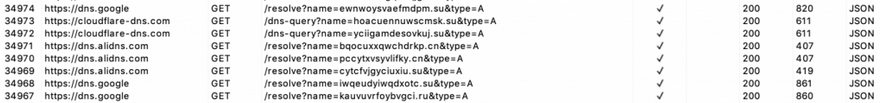
\includegraphics[scale=0.51]{dns.png} 
\end{center}
Der gesamte Source Code der dies möglich macht liegt in der heruntergeladenen APK. In späteren Versionen wurde der eigentliche Payload in  Form der Phishing Malware erst nachträglich über den C\&C geladen. Hierbei wird ein GET Request für die benötigten Dateien gestellt. Jegliche Kommunikation zwischen Gerät und Server wird anhand RSA verschlüsselt.
\newpage
\subsection{Payload}
Die Payload als auch die restliche APK von Flubot sind komplett in JAVA geschrieben. Sie enthält den benötigten Source Code um Kontakt zu dem C\&C Server herzustellen, die benötigten Berechtigungen einzufordern und die Phishing Malware auf ausgewählte Applikationen anzuwenden. Auch die RSA keys für die verschlüsselte Kommunikation sind enthalten. Die gepackte APK welche den Payload trägt ist anhand MD5 gehashed und wird erst auf dem Gerät entpackt. Genauer betrachtet ist ein Android Application Package die  Installations Datei für eine Android App. In ihr befinden sich alle benötigten Dateien für die Installation und Ausführung der Anwendung. In Grunde genommen ist eine Apk eine Kompromitierte zip Datei die auch mit bekannter Software wie Winrar geöffnet werden kann. Das gleiche gilt  für Flubot. Um sicherheitsanalysen jedoch zu erschweren verwendet die Malware sogenannte String Obfuscation. Dies ist ein Konzept dessen Hauptaufgabe darin besteht Programmcode zu verschleiern bzw. unleserlich zu machen. Dies wird beispielweise durch Variablensubsitution erreicht. Teilweise werden auch komplette Codeabschnitte verschlüsselt. Für die Obfuscation verwendet Flubot das Open Source tool paranoid!
Durch Reverse Engineering gelang es den Code zu Deobfuscieren also wieder leserlich zu machen. 
Die Datei AndroidManifest.xml enthält alle Berechtigungen die eine APK benötigt. Flubot hat über 40 Einträge die unter anderem Internet Zugriff und das versenden von SMS autorisieren. 
\begin{shaded}
android.permission. READCONTACTS\\
permission. WRITESMS\\
permission. INTERNET
\end{shaded}
Des weiteren ist es gelungen die Kommunikationskommandos zwischen Malware und  des Command and control servers zu erfassen. Derzeit sind über 20 Kommandos möglich, wobei Flubot stetig weiterentwickelt und um Funktionalitäten ergänzt wird.
\begin{center}
 Kommandos von dem C\&C Server an das Gerät
\end{center}

\begin{shaded}
GETCONTACTS - Send contact list to server. Later its used for spamming\\
RETRYINJECT
\end{shaded}
\begin{center}
 Kommandos von Gerät an Server
\end{center}
\begin{shaded}
GET SMS Get the phishing SMS text including phone number\\
GET INJECTS LIST Get the list of targeted applications by sending all package names.\\
GET INJECT Fordert den Html code für das jeweilige Phishing overlay an.
\end{shaded}
\newpage
Die APK ist n mb groß und enthählt mehrere tausend Zeilen Code.\\
Die eigentliche Phishing Attacke welche ein Overlay über die betroffene Anwendung legt, wird mittels Webview umgesetzt. Das heißt bei öffnung der infizierten app wird das overlay mittels html code im browser dargestellt und über die Anwendung gelegt.
\begin{shaded}
 \begin{lstlisting}
 private void LoadHtml() {
  String GetInject = Bot.GetInject(packagename);
  #package name wird durch die geziele Application ersetzt.
   if (GetInject==0) {
	finishandRemovetask();
	 }   else {
	this.webView.loadDataWithBaseURL(null, GetInject,
	Deobfuskator$app$Release.getString(-225216466544654L);
	Deobfuskator$app$Release.getString(-225216466544654L);
	null;
	)
 }
}
\end{lstlisting}

\end{shaded}
Flubot wird stetig weiterentwickelt und gewinnt zunehmend an Komplexität. Technisch ist die Malware auf dem neuesten Entwicklungsstand und auch aufgrund der Größe höchstwahrscheinlich von einem größeren Team professionell entwickelt worden.  




\newpage
\section{Lösungsansätze}
Flubot hat einige Mechanismen implementiert um nicht erkannt und entfernt zu werden. So wird die Anwendung nicht unter installierter Software gelistet und ist auch in einigen Taskmanagern nicht als Prozess sichtbar. Findet man die Installationsdatei doch, blockiert Flubot den Andriod deinstaller.  Des weiteren ist Flubot in der Lage 'Play protect' zu deaktivieren. Dennoch ist die Entfernung der Malware durch Rücksetzung zum Werkzustand recht einfach. Dies hat allerdings ein Verlust der persönlichen Daten zur Folge. Eine Entfernung ohne Datenverlust ist beispielweise durch das Open-Source tool malninstall
möglich. Dieses Tool wurde speziell für die Entfernung von Flubot entwickelt.\\
Grundsätzlich gibt es kein generelle technische Lösung gegen Phishing Malware. Da solch Angriffe in erster linie Social Engineering nutzen ist es schwierig ein technischen Mittel dagegen zu entwickeln. Der Mensch ist immer der anfälligste Teil eines Sicherheitsrelevanten Systems. Ein gewisser Schutz bietet jedoch Zwei Faktor Authentifizierung, der wenn möglich in allen Anwendungen aktiviert sein sollte!\\ Das größtmögliche Potential stellt eine bessere Bildung und Aufklärung da! Informatik sollte in Schulen deutlich stärker gewichtet werden und auch It Sicherheitsrelevante Themen lehren!
\section{Ausblick und Conclusion}
Phishing ist nach wie vor die meist verwendete Angirfssmethode.
Die gruppierung wurde im Herbst 2021 in Spanien festgesetzt. Das Botnetzt verbreitet sich allerdings nach wie vor!
\end{document}

